\documentclass[a4paper]{article}
\usepackage{graphicx,amssymb} 
\usepackage{amsmath,bm,bbm}
%\usepackage{hyperref}
%\usepackage{cite}
\usepackage[binary-units]{siunitx}
\usepackage[square,sort]{natbib}
\usepackage[left=35mm, right=35mm, top=15mm, bottom=20mm, noheadfoot]{geometry}

\textwidth=15cm \hoffset=-1.2cm 
\textheight=25cm \voffset=2cm 


\pagestyle{empty} 

\date{} 

\def\keywords#1{{\bf Keywords: }{#1}}

\begin{document}
\thispagestyle{empty}

\title{\textbf{An Exploratory Study of the Transition Graphs Application in SAR Textures}}

\author{Eduarda T. C. Chagas, Heitor S.\ Ramos \\ 
	Departamento de Ci\^encia da Computa\c c\~ao, Universidade Federal de Minas Gerais \\ \\ 
	
	Osvaldo A.\ Rosso, \\
	Instituto de F\'isica, Universidade Federal de Alagoas\\ \\
	
	Alejandro C.\ Frery \\
	School of Mathematics and Statistics, Victoria University of Wellington
}

\date{}
\maketitle\thispagestyle{empty} 

\begin{abstract}

A new perspective on the analysis of surfaces and land use has been carried out with the synthetic aperture images (SAR) extraction and classification.
With the popularization of machine and deep learning techniques, such algorithms have revolutionized the performance and interpretability of their results~\citep {han2020unsupervised, huang2020classification, xie2020polsar}.

On the other hand, in the context of non-parametric time series analysis, the methodology of~\cite{PermutationEntropyBandtPompe} has been used successfully in several areas of scientific knowledge~\citep{baravalle2018discriminating, Araujo2019permutation, ClassificationVerificationOnlineHandwrittenSignatures}.
Obtaining a new representation of the time series through the ordinal patterns, the distributions resulting from the histogram of frequencies or from the pattern transition graphs become less sensitive to outliers and do not assume any hypothesis about the nature of the data.
Despite its simplicity, this method is robust to noise, has a low computational cost and when used in conjunction with causal descriptors from the Information Theory, it has been showing good results in the signals characterization and classification.

In this context, the work developed by~\citet{ChagasClassification2020} proposes an applicability expansion of this methodology in the remote sensing context, presenting a new perspective of extracting characteristics in textures from SAR images.
For that, it was necessary to perform the dimensionality reduction transforming the patch of homogeneous textures \mbox{2-D} into a signal \mbox{1-D} through the Hilbert-Peano curves~\citep{Lee1994Texture} .
With this approach, it was found that it is possible to preserve relevant properties of spatial pixel correlation (since such a curve never maintains the same orientation for more than three consecutive points) with a low computational cost.

However, the main contribution of this work consists in the modification proposal of the ordinal patterns transition graphs, called weighted amplitude transition graph (WATG), in such a way that it was able to discriminate similar patterns with different intensity variations.
Once the probability distribution of the transitions between the symbols is obtained, it is through the Information Theory descriptors that important characteristics of the underlying process are revealed, having interpretability in terms of the spatial dependence between the observations.
These descriptors are Shannon's Entropy and Statistical Complexity.

The first descriptor is a measure of the system's disorder, and is defined as
\begin{equation}
	H(\mathbbm{P}) = -\frac{1}{\log D!} \sum_{\ell=1}^{D!^2} \Big(p_\ell \log p_\ell\Big),
\end{equation}
where $D$ represents the dimension of the ordinal patterns used in the symbolization process, and $\mathbbm{P} = \{p_{(\widetilde\pi^D_1, \widetilde\pi^D_1)}, p_{(\widetilde\pi^D_1, \widetilde\pi^D_2)}, \dots, p_{(\widetilde\pi^D_{D!}, \widetilde\pi^D_{D!})} \} = \{p_1,\dots,p_{D!^2}\}$ is the probability distribution obtained of the image patch when WATG is applied.

Although very expressive, the Normalized Shannon Entropy is not able to describe all possible underlying dynamics.
To this aim, \citet{LopezRuiz1995} proposed using the disequilibrium  $Q$, a measure of how far $\mathbbm{P}$ is from an equilibrium or non-informative distribution $\mathbbm{U}$.
It is calculated as:
\begin{equation}
Q'(\mathbbm{P}, \mathbbm{U}) = \sum_{\ell=1}^{D!^2} \Big(p_\ell \log\frac{p_\ell}{u_\ell} +
u_\ell \log\frac{u_\ell}{p_\ell}
\Big),
\end{equation}
where our normalized formula is $Q = Q'/\max\{Q'\}$.
With this, they proposed the Statistical Complexity $C = HQ$ which measures the dependence structures among the elements.
So, a sequence can be mapped into a point $(h,c)$, and the set of all possible point is the Entropy-Complexity plane (or $H\times C$ plane).
Fig.~\ref{fig:Outline}, shows the outline of the methodology proposed in~\citet{ChagasClassification2020}.


When each patch of UAVSAR images is represented as a point in the Entropy-complexity plane (or HC plane), a perfect separation between urban, pasture, ocean and forest areas is observed.
In addition to presenting a better performance than the analyzed baselines, this characterization has some advantages:
~(i) provides easy visualization of features and
~(ii) your training process with machine learning algorithms becomes faster and less costly.

The intensity of the SAR texture signals is directly related to the analyzed targets nature and their backscattering properties.
Therefore, the study of the such pixels spatial structure using consolidated techniques in non-parametric analysis of time series represents a fruitful field of investigation.

In this context, we seek to analyze WATG in new scenarios for the classification of homogeneous textures, in which the following research questions stand out:

~(i) What is the impact of the dimensions variation of Hilbert curves on the final descriptors?
When characterizing and classifying SAR images, the application of Hilbert-Peano curves with dimensions equal to $128 \times 128$ is suggested.
Thus, the objective of this experiment is to analyze the minimum dimension necessary to obtain a good characterization when we apply WATG in textures of SAR images;

~(ii) Can we observe variations in the results when we apply other backscatter bands?
Since WATG is investigated only with polarimetric SAR quad images with HHHH backscatter magnitudes, here we conduct an investigation as to its use in other magnitudes and their impact on the HC plane;

~(iii) How does the algorithm behave when exposed to different surfaces?
For this, we selected new L-band polarimetric SAR images with HHHH backscatter magnitudes from the unmanned aerial vehicle synthetic radar sensor (UAVSAR) of the NASA Jet Propulsion Laboratory (JPL).
A new dataset was built with $700$ images patches and the same dimensions used in the previous work for Hilbert-Peano curves, containing the following classes: pasture, forest, oceans, glacial, desert and urban regions.

\begin{figure}
	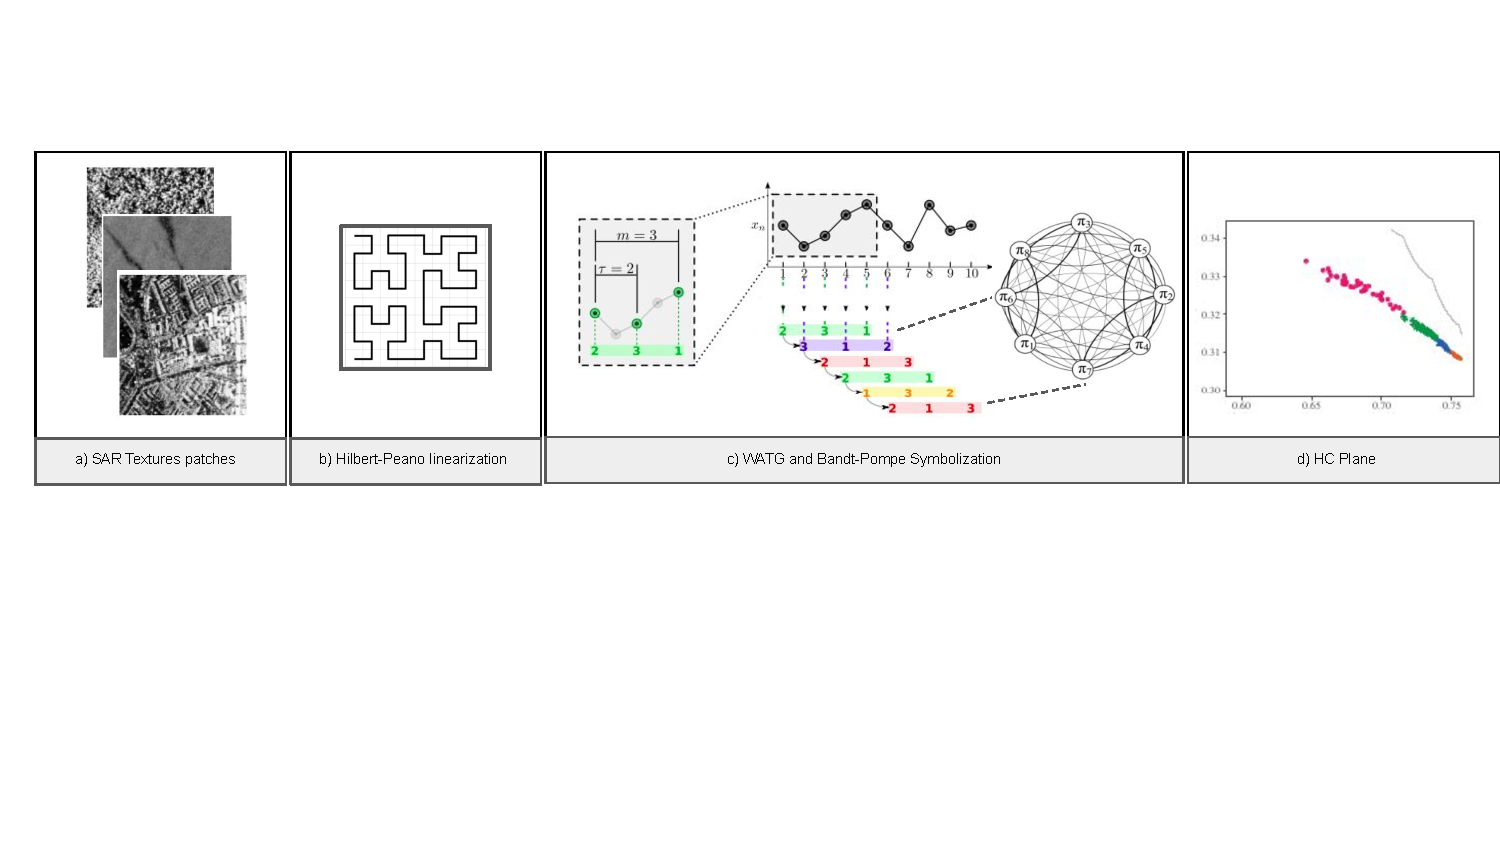
\includegraphics[width=\columnwidth]{SARTexture.pdf}
	\caption{Outline of the methodology used for the textures classification.}
	\label{fig:Outline}
\end{figure} 

\end{abstract}

\keywords{
    Synthetic Aperture Radar (SAR), 
	Terrain Classification,		
	Information Theory, 
	Ordinal Patterns.
}

\bibliographystyle{unsrtnat}
\bibliography{ref}

\end{document}